%%%%%%%%%%%%%%%%%%%%%%%%%%%%%%%%%%%%%%%%%%%%%%%%%%%%%%%%%%%%%%%%%%%%%%%%%%%%%%%
% CAP�TULO 2
\chapter{FUNDAMENTA��O TE�RICA}  

O cap�tulo de Fundamenta��o Te�rica deve definir os principais conceitos do trabalho e apontar os trabalhos relacionados. Cont�m a exposi��o ordenada e pormenorizada do assunto. � composta de revis�o de literatura, dividida em se��es e subse��es descritas detalhadamente. Cada se��o ou subse��o dever� ter um t�tulo apropriado ao conte�do. 

A seguir ilustra-se a forma de incluir figuras, tabelas, equa\c{c}\~oes, siglas e s\'imbolos no documento, obtendo indexa\c{c}\~ao autom\'atica em suas respectivas listas. A numera\c{c}\~ao sequencial de figuras, tabelas e equa\c{c}\~oes ocorre de modo autom\'atico. Refer\^encias cruzadas s\~ao obtidas atrav\'es dos comandos {\ttfamily \textbackslash label\{\}} e {\ttfamily \textbackslash ref\{\}}. Por exemplo, n\~ao \'e necess\'ario saber que o n\'umero deste cap\'itulo \'e~\ref{chap:desenv} para colocar o seu n\'umero no texto. Isto facilita muito a inser\c{c}\~ao, remo\c{c}\~ao ou reloca\c{c}\~ao de elementos numerados no texto (fato corriqueiro na escrita e corre\c{c}\~ao de um documento acad\^emico) sem a necessidade de renumer\'a-los todos.

\section{Figuras}

Na figura~\ref{fig:dummy} \'e apresentado um exemplo de gr\'afico flutuante. Esta figura aparece automaticamente na lista de figuras. Para uso avan\c{c}ado de gr\'aficos no \LaTeX, recomenda-se a consulta de literatura especializada~\cite{Goossens2007}.


\begin{figure}[!htb]
	\centering
	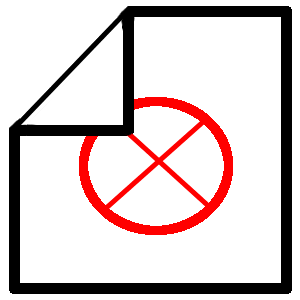
\includegraphics[width=0.2\textwidth]{./Figuras/dummy.png} % <- formatos PNG, JPG e PDF
	\caption[Exemplo de uma figura]{Exemplo de uma figura onde aparece uma imagem sem nenhum significado especial.}
	\fonte{\cite{abnTeX2009}}
	\label{fig:dummy}
\end{figure}


\section{Tabelas}

Tamb\'em \'e apresentado o exemplo da tabela~\ref{tab:correlacao}, que aparece automaticamente na lista de tabelas. Informa\c{c}\~oes sobre a constru\c{c}\~ao de tabelas no \LaTeX\ podem ser encontradas na literatura especializada~\cite{Lamport1986,Buerger1989,Kopka2003,Mittelbach2004}.

\begin{table}[!htb]
	\centering
	\caption[Exemplo de uma tabela]{Exemplo de uma tabela mostrando a correla\c{c}\~ao entre x e y.}
	\label{tab:correlacao}
	\begin{tabular}{cc}
		\hline 
		x & y \\
		\hline
		1 & 2 \\
		3 & 4 \\
		5 & 6 \\
		7 & 8 \\
		\hline 
	\end{tabular}
	\fonte{Autoria pr\'opria.}
\end{table}

\section{Equa\c{c}\~oes}

A transformada de Laplace \'e dada na equa\c{c}\~ao~(\ref{eq:laplace}), enquanto a equa\c{c}\~ao~(\ref{eq:dft}) apresenta a formula\c{c}\~ao da transformada discreta de Fourier bidimensional\footnote{Deve-se reparar na formata\c{c}\~ao esteticamente perfeita destas equa\c{c}\~oes!}.

\begin{equation}
X(s) = \int\limits_{t = -\infty}^{\infty} x(t) \, \text{e}^{-st} \, dt
\label{eq:laplace}
\end{equation}

\begin{equation}
F(u, v) = \sum_{m = 0}^{M - 1} \sum_{n = 0}^{N - 1} f(m, n) \exp \left[ -j 2 \pi \left( \frac{u m}{M} + \frac{v n}{N} \right) \right]
\label{eq:dft}
\end{equation}

\section{Siglas e s\'imbolos}

O pacote \textsc{abn}\TeX\ permite ainda a defini\c{c}\~ao de siglas e s\'imbolos com indexa\c{c}\~ao autom\'atica atrav\'es dos comandos {\ttfamily \textbackslash sigla\{\}\{\}} e {\ttfamily \textbackslash simbolo\{\}\{\}}. Por exemplo, o significado das siglas\sigla{CPGEI}{Programa de P\'os-gradua\c{c}\~ao em Engenharia El\'etrica e Inform\'atica Industrial},\sigla{DAELN}{Departamento Acad\^emico de Eletr\^onica} e\sigla{UTFPR}{Universidade Tecnol\'ogica Federal do Paran\'a} aparecem automaticamente na lista de siglas, bem como o significado dos s\'imbolos\simbolo{$\lambda$}{comprimento de onda},\simbolo{$v$}{velocidade} e\simbolo{$f$}{frequ\^encia} aparecem automaticamente na lista de s\'imbolos. Mais detalhes sobre o uso destes e outros comandos do \textsc{abn}\TeX\ s\~ao encontrados na sua documenta\c{c}\~ao espec\'ifica~\cite{abnTeX2009}.

